\section{Method}
\label{sec:method}

\subsection{Spectral decay model}

Let $\mathbf{W} \in \mathbb{R}^{C_{out} \times C_{in} k^2}$ be the flattened kernel of a
convolutional layer and let $\sigma_1 \ge \sigma_2 \ge \cdots \ge \sigma_r$ be its
singular values. We model the decay as a power law with an additive noise floor:

\begin{equation}
\label{eq:decay}
\sigma_i^2 = A i^{-\beta} + \eta^2, \qquad i = 1, \dots, r,
\end{equation}

where $\eta$ is the standard deviation of the calibration residual. Fitting
Equation~\eqref{eq:decay} by least squares over the first $r$ singular values yields
$(\hat{A}, \hat{\beta}, \hat{\eta})$.

\subsection{Truncation rank}

Given the fitted parameters, the energy retained by keeping the first $k$ components is

\begin{align}
\label{eq:retained}
E(k) &= \frac{\sum_{i \le k} \sigma_i^2}{\sum_{i \le r} \sigma_i^2}, \\
\label{eq:rank}
k^\star &= \argmin_{k} \; \bigl[\, \lambda\,(1 - E(k)) + (1 - \lambda)\, k / r \,\bigr],
\end{align}

with $\lambda$ a Lagrange multiplier trading accuracy against computation. We set
$\lambda = 0.85$ in all experiments; Figure~\ref{fig:pipeline} shows the pipeline and
Figure~\ref{fig:sensitivity} reports the sensitivity to this choice.

\begin{figure}[t]
  \centering
  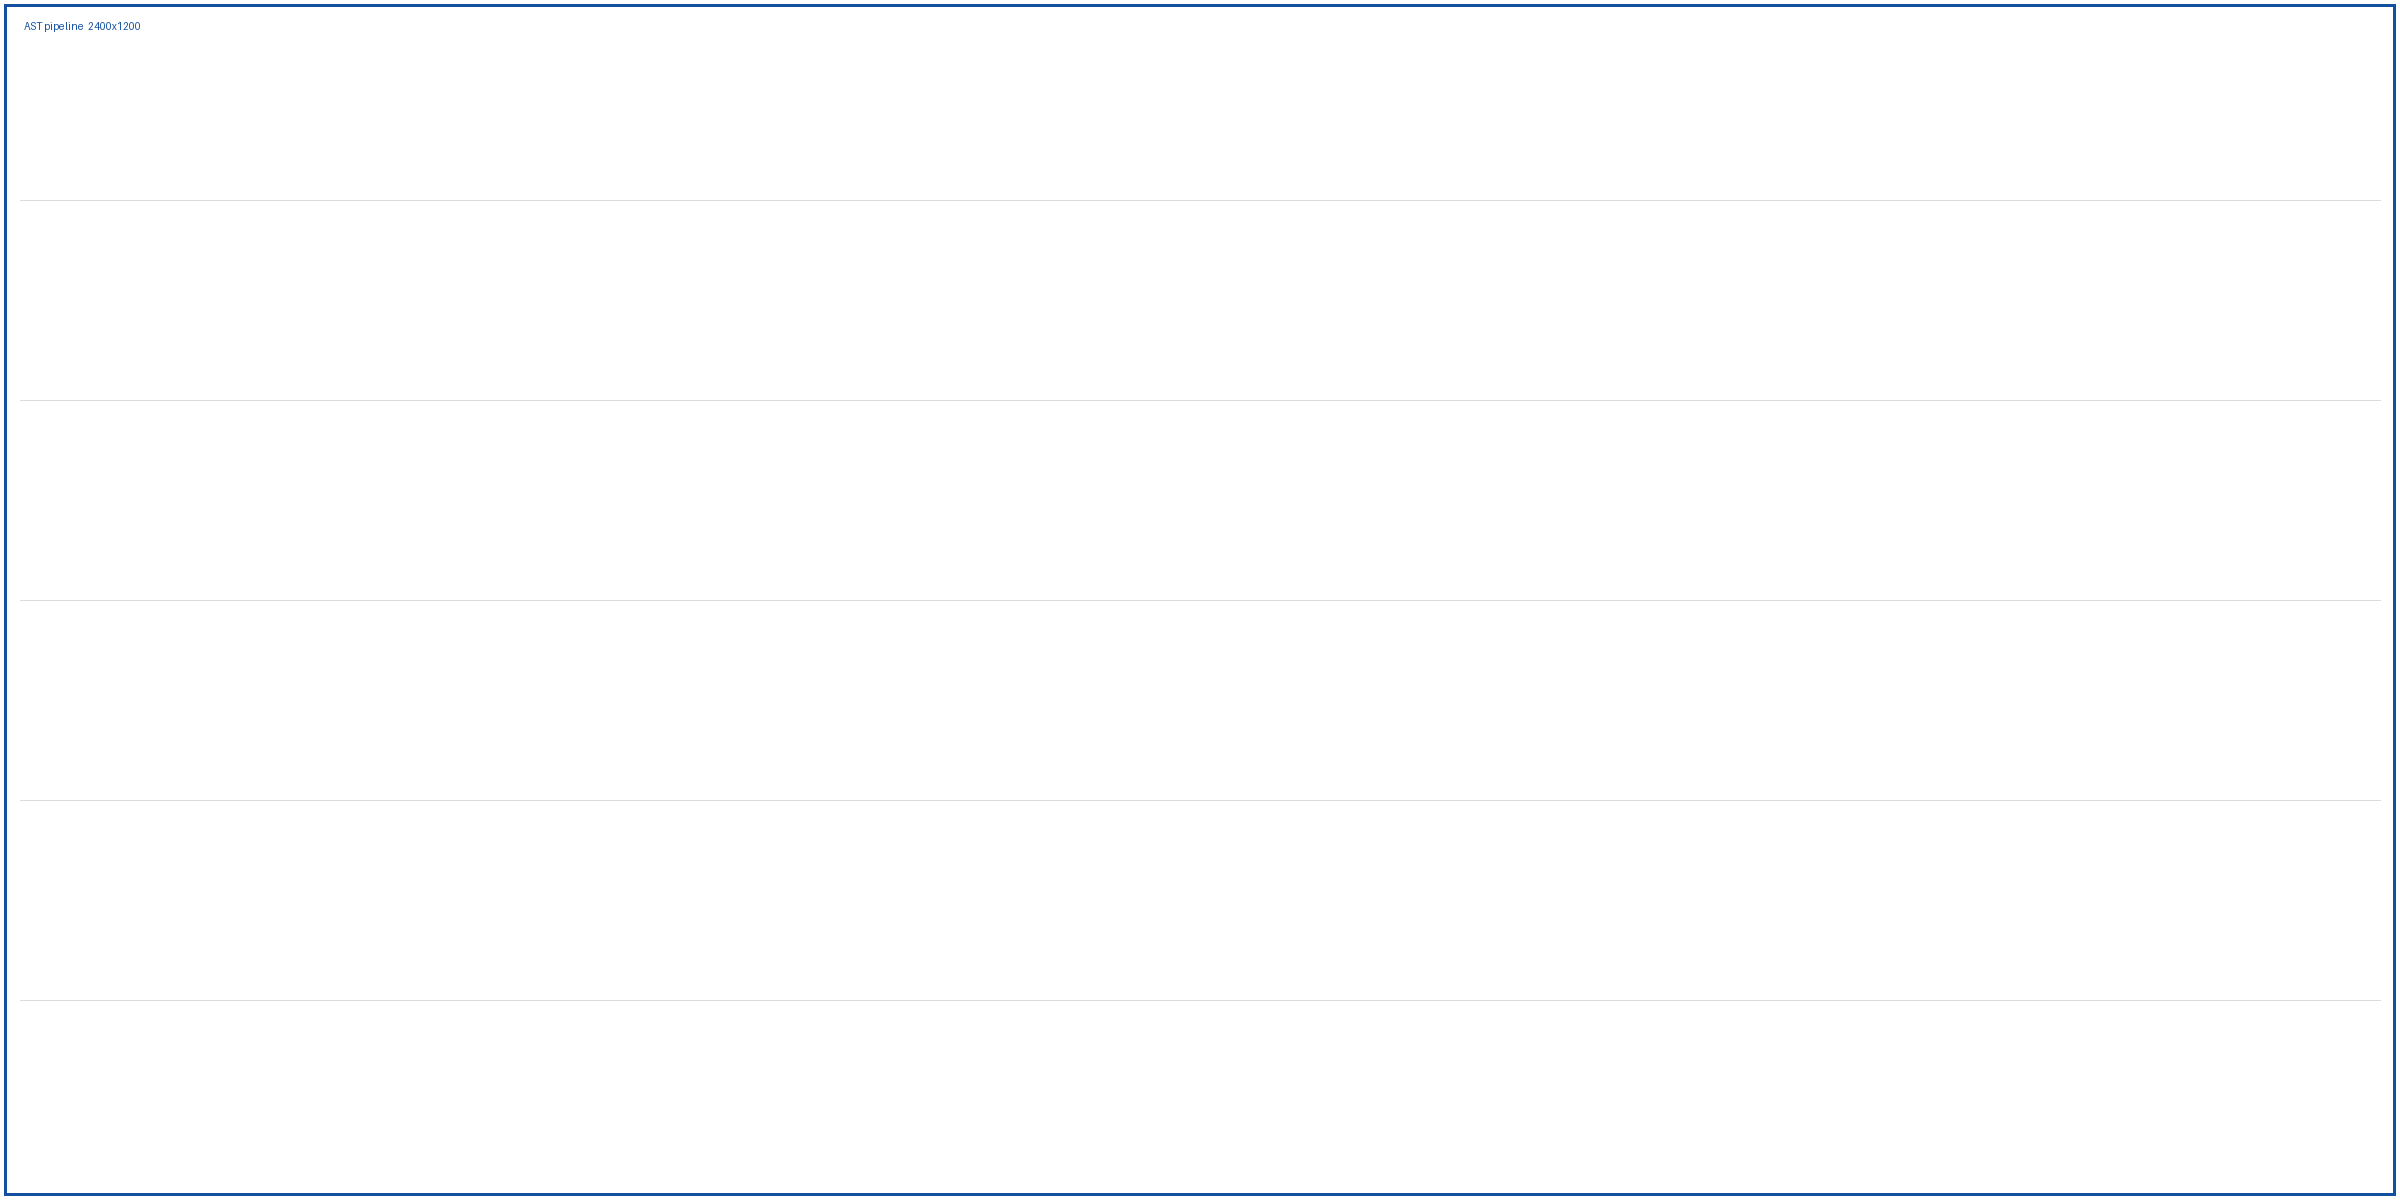
\includegraphics[width=\linewidth]{figures/pipeline.png}
  \caption{Overview of \method{}. Calibration data is passed through the frozen network;
  per-layer singular spectra are fitted to Equation~\eqref{eq:decay}; the resulting rank
  mask is folded into the convolution at export time.}
  \label{fig:pipeline}
\end{figure}

\begin{figure}[t]
  \centering
  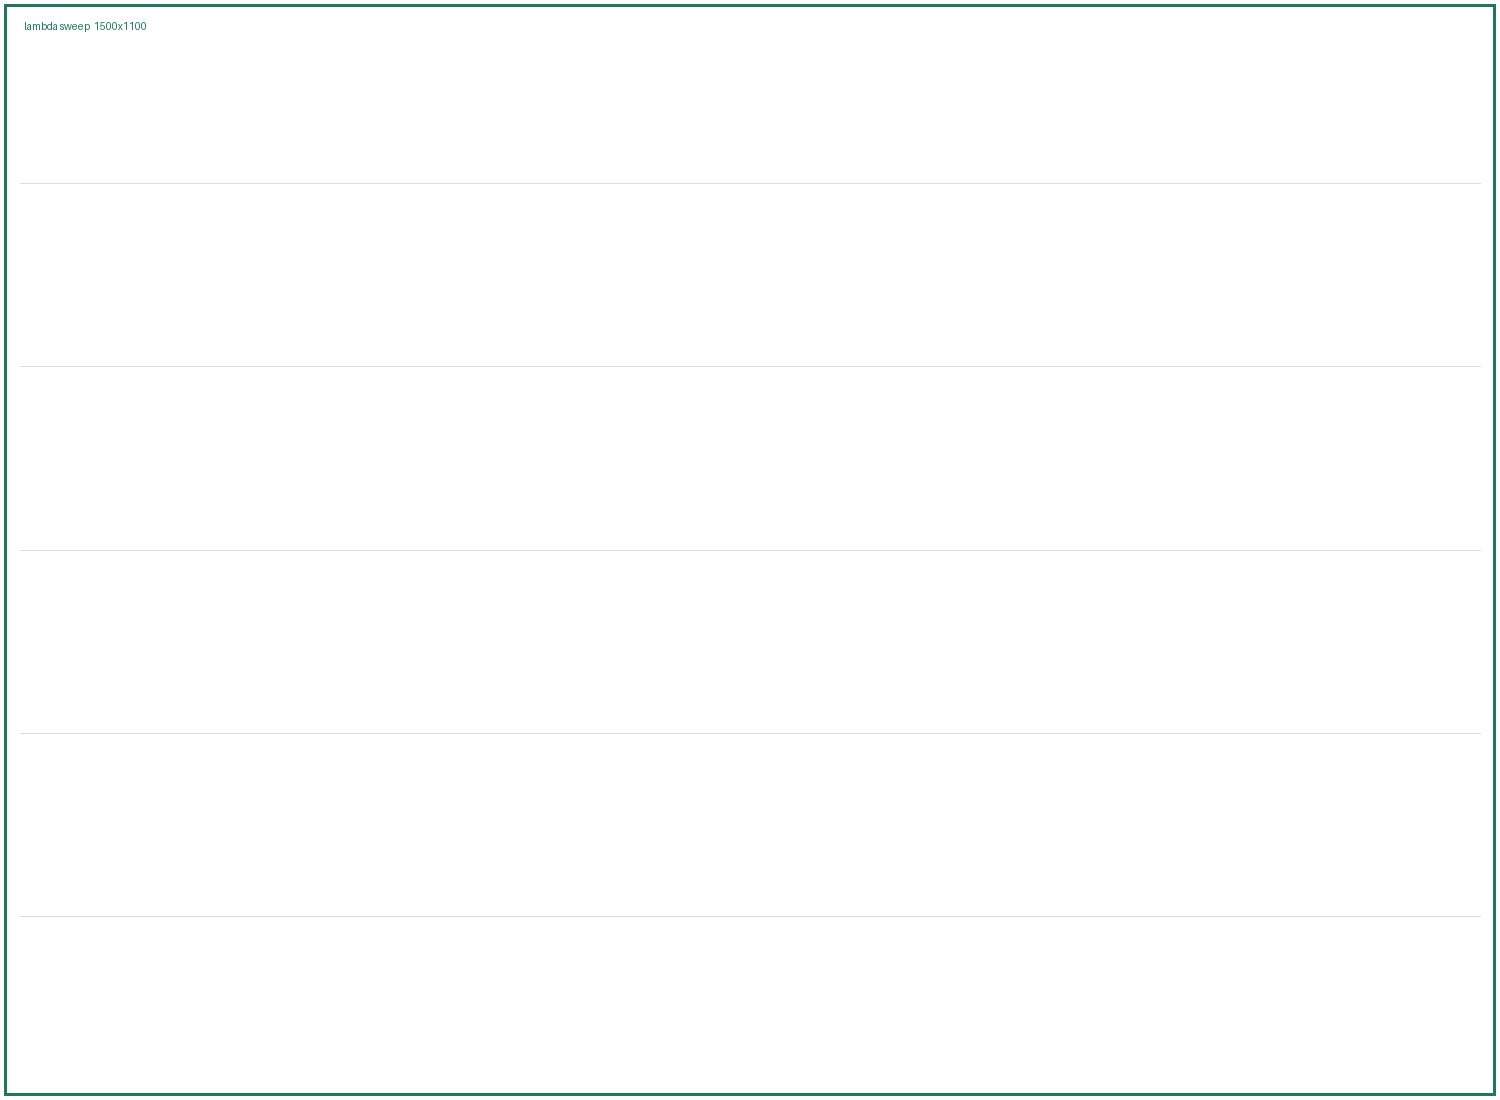
\includegraphics[width=0.48\linewidth]{figures/sensitivity.png}
  \caption{Sensitivity of top-1 accuracy to the multiplier $\lambda$.}
  \label{fig:sensitivity}
\end{figure}

\subsection{Complexity}

The additional cost of calibration is $O(r)$ per layer and is dominated by the
one-time SVD, as summarized in Table~\ref{tab:complexity}.

\begin{table}[t]
  \centering
  \caption{Per-layer calibration cost for the ResNet-18 backbone.}
  \label{tab:complexity}
  \begin{tabular}{lrrr}
    \toprule
    Stage & Params (M) & SVD (ms) & Peak RAM (MB) \\
    \midrule
    Stem        & 0.009 & 4.1  & 3.2  \\
    Stage 1     & 0.147 & 22.8 & 11.5 \\
    Stage 2     & 0.525 & 88.3 & 40.1 \\
    Stage 3     & 2.100 & 301.7 & 158.4 \\
    Stage 4     & 8.400 & 1187.2 & 612.9 \\
    \bottomrule
  \end{tabular}
  \tnote{Measured on a single Intel Xeon Gold 6248 core at 2.5~GHz.}
\end{table}
